\subsubsection{Video Streaming}
\label{subsubsec:video-streaming}
% nur möglichkeit, erweiterung in kap 6
% Websockets in Webseite und App
% Welche /dev/ sind vorhanden
% Wer kümmert sich? Pi oder Nanos etc

Der \gls{go1} bietet mit seinen fünf Kameras die Möglichkeit, Bilder seiner Umgebung zu übertragen und es den Nutzern so
zu ermöglichen, den Roboter aus der Entfernung zu steuern.
Die Positionierung, Verteilung und die Mounting-Points der Kameras innerhalb des Roboters, den Recheneinheiten und den
Betriebssystemen wurde bereits in Kapitel \ref{subsec:hardware-architektur} geschildert.
Kurz zusammengefasst sind im Kopf des Roboters zwei Kameras positioniert, nach vorne und nach unten gerichtet.
Beide sind am Jetson Nano innerhalb des Kopfes verbunden.
Die beiden Außenseiten des Rumpfes sind mit zwei Kameras bestückt, die mit dem Jetson Nano m Rumpf des \gls{go1} verbunden sind.
Die letzte Kamera an der Unterseite des Rumpfes ist mit dem Jetson Xavier NX verbunden.
Am Beispiel der nach vorne gerichteten Kamera im Kopf des \gls{go1} soll in diesem Kapitel kurz erläutert werden,
wie auf die Kameras zugegriffen werden kann und wie man von einem verbundenen Rechner außerhalb des Roboters auf die Bilder
zugreifen kann.
Die dargestellte Anleitung ist für alle anderen Kameras bis auf etwaige Mounting-Points und \gls{ip} Adressen identisch.

\myparagraph{Zugriff auf Kamerabilder}

Um die Kameras des \gls{go1} nutzen zu können, müssen zuerst alle Prozesse gestoppt werden, die die Geräte selbst blockieren.
Geprüft werden kann dies über den Befehl \texttt{fuser -vm /dev/\allowbreak video1}, hier muss nach der Ausgabe nach den Zeilen gesucht werden,
die als \texttt{ACCESS}-Flag den Wert \texttt{m} für \texttt{memory mapped files} haben.
Die Prozesse können dann mit deren Namen beendet werden.

\begin{lstlisting}[language=Bash]
pkill -f point_cloud_nod
pkill -f example_point
\end{lstlisting}

\noindent Für den Zugriff auf die Daten der Kamera über den Mount-Point \texttt{/dev/\allowbreak video1} kann das Paket \texttt{ffmpeg}
genutzt werden, das auf allen Ubuntu Systemen des \gls{go1} vorinstalliert ist.
Folgender Befehl inklusive Erläuterung zu den Optionen kann genutzt werden, um per \texttt{ffmpeg} einen Videostream
über \gls{rtsp} auf einen Streaming-Server zu starten.

\begin{lstlisting}[language=Bash]
ffmpeg -nostdin \                  # Keine Interaktion
    -f video4linux2 \              # Input Format
    -i /dev/video1 \               # Input-URL
    -vcodec libx264 \              # Video Kodierung (h264)
    -preset:v ultrafast \          # Kodierungsgeschwindigkeit
    -tune zerolatency \            # Keine H264 B-Frames
    -framerate 5 \                 # Framerate
    -f rtsp \                      # Output Format
    rtsp://<ip:8554|port>/<stream> # Output File/URL
\end{lstlisting}

\noindent Weitere Details zur Ausführung und dem Streaming über einen Server werden in Kapitel \ref{sec:funktionserweiterungen-und-integration}
behandelt.
Das Kamerabild ist beim Streaming über \texttt{ffmpeg} in keiner Form verarbeitet und sieht wie in Abbildung \ref{fig:kamera-bild}
dargestellt aus.

\begin{figure}[h]
    \frame{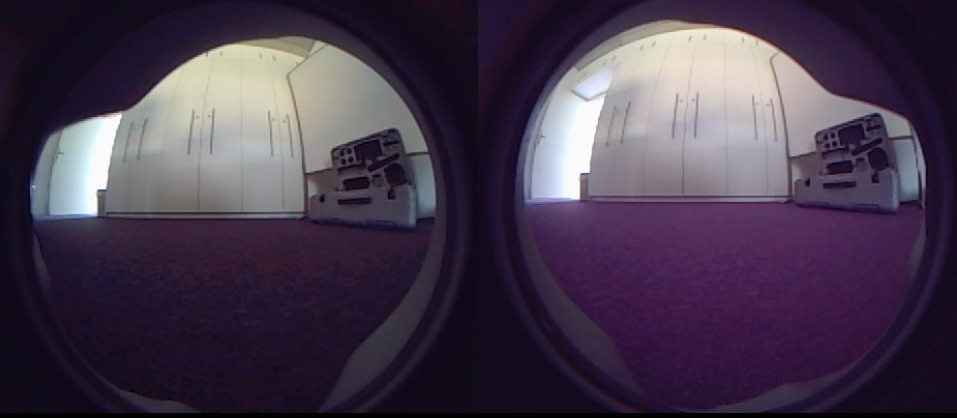
\includegraphics[width=\linewidth]{img/analyse/kamera-bild}}
    \caption{Kamerabild des GO1}\label{fig:kamera-bild}
\end{figure}

Eine Verarbeitung und Verbindung der beiden \emph{Fischaugen} der Kamerabilder ist im Roboter bereits mit der Bibliothek \emph{OpenCV}
umgesetzt.
Auch die in Kapitel \ref{subsubsec:ressourcen} genannte \emph{Unitree-Camera-SDK} nutzt OpenCV in der Implementierung.
Im Rahmen dieser Arbeit wird jedoch nicht auf die erweiterten Funktionen durch den Einsatz von OpenCV eingegangen.
Hierfür kann die Arbeit \citetitle{jonas}\footcite{jonas} zu Rate gezogen werden.